\chapter{Results and Discussion}
The results of our experiments with our data set will be presented in this chapter. 30 runs of each approach that produced feasible solutions are included in the results. Note that some runs produce an infeasible solution. This due to the non-deterministic nature of metaheuristics, which will cause it to produce infeasible solutions sometimes.

\section{Environment}
All of the approaches were run in the following hardware and software configurations:

\begin{itemize}
	\item Hardware
	\begin{itemize}
		\item \textbf{CPU}: Intel Core i3-5010U @ 2.1GHz
		\item \textbf{GPU}: NVIDIA GeForce 920M
		\item \textbf{RAM}: 4GB
	\end{itemize}
	\item Software
	\begin{itemize}
		\item \textbf{OS}: elementaryOS 5.1.7 Hera
		\item \textbf{Linux Kernel Version}: 5.4.0-80-generic
	\end{itemize}
\end{itemize}

\section{Experiments}
Each approach has their own parameters, and the values we have set for those parameters are shown in Table \ref{approach-parameters}. Both approaches use a population size of 50, and a maximum number of iterations of 400. The following parameter values for the PSO approach were taken from the work of Jolai, F., Tavakkoli-Moghaddam, R., and Taghipour, M. \cite{Jolai2012}.

\begin{table}[h!]
	\centering
	\begin{tabular}{|l|l|l|}
		\hline
		\textbf{Approach}   & \textbf{Parameter} & \textbf{Value} \\ \hline
		GWO                 & c                  & 4              \\ \hline
		\multirow{3}{*}{GA} & Mutation Rate      & 0.05           \\ \cline{2-3} 
		& Tournament Size    & 4              \\ \cline{2-3} 
		& No. of Elites (EN) & 5              \\ \hline
		\multirow{3}{*}{PSO} & w      & 0.05           \\ \cline{2-3} 
		& c1    & 2              \\ \cline{2-3} 
		& c2 	& 2              \\ \hline
	\end{tabular}
	\caption{Parameter values of the GWO, GA, and PSO approaches.}
	\label{approach-parameters}
\end{table}

The results obtained for each approach is shown in Tables \ref{approach-ga-results}, \ref{approach-gwo-results}, and \ref{approach-pso-results}, respectively. As what the tables show, the competing genetic algorithm approach produces a solution that is better than our proposed GWO approach and the PSO approach, with a fitness averages of $273.537430766667$, $50422.3174052667$, and $88087.9226730667$ for the SFLP-II, mSFLP-III, and mKra30a problem configurations respectively. This is compared to our proposed approach's fitness averages of $290.3857809$, $52702.9314929$, $101874.328208933$. Fortunately for our approach, the PSO approach obtained the fitness averages of $324.356679733333$, $64181.9165261333$, and $118785.277772567$, proving that our GWO is not the worst approach. For SFLP-II, the best and worst solutions have fitnesses of $221.042599$ and $324.874681$ for the GA, respectively, compared to our approach's $234.250481$ and $339.099181$. The PSO approach obtained $268.59568$ and $380.688077$s. In this data set, our approach was capable of producing the best solution. For mSFLP-III, the best and worst solutions have a fitness of $46802.666237$ and $53474.353325$ for the GA, respectively, compared to our approach's $48951.787331$ and $53474.353325$ and the PSO approach's $60037.826591$ and $68194.108383$. Lastly, for mKra30a, the best and worst solutions have fitnesses of $76651.01432$ and $98512.468674$, respectively, with our approach obtaining $90455.74585$ and $118315.534424$. PSO produces the poorest best and worst solutions with fitnesses of $106178.045845$ and $130915.770554$. From the results, the competing GA approach is the most stable among the three, basing from the lower standard deviation in all data sets, with $25.3555205871573$, $1630.42444301206$, and $5077.72744984237$ for SFLP-II, mSFLP-III, and mKra30a, respectively. This is compared to our approach's $32.4373567833344$, $2224.64491886288$, and $7190.18569614101$, and the PSO approach's $38.4539160542525$, $1956.45733138936$, and $6138.39410532314$. This behaviour of producing the best average solution of the GA approach is attributed to the local search methods, which relatively exhaustively finds a better solution in a small area near the best solution found so far in each iteration. These local search methods intensifies the exploitation phase of the approach. Our GWO approach also exploits the local area, but it is not as intensive as the GA approach and only occurs at a later time in a run, similar to how the PSO approach behaves. Notice as well how PSO produces the worst solutions on average among the three. This can be explained with how particles in the PSO approach are equally influenced by their personal best position and their swarm's global best position. This reduces the chances of particles from exploiting the area around the global best position. This is unlike our GWO approach where all wolves are influenced/led by the best three wolves, enabling them to exploit the space around the best found solution. In future studies, different behaviour may be observed when the PSO parameters are tweaked to different values.

\begin{figure}[h!]
\centering
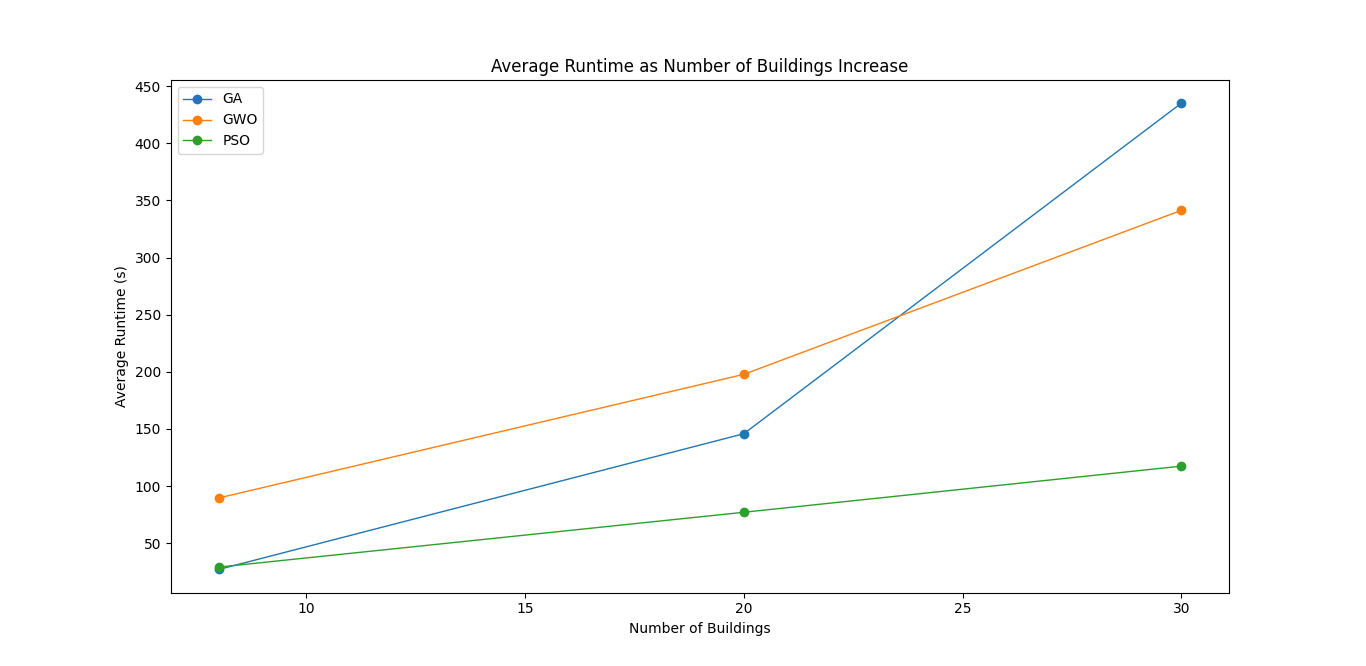
\includegraphics[scale=0.65]{./images/chap07-rd/approaches-average-runtime-over-no-of-buildings.png}
\caption{The average runtime (s) of each of the approaches as the number of buildings in a data set increase.}
\label{graph-approaches-runtime-no-buildings}
\end{figure}

The genetic algorithm approach is also faster when SFLP-II is being used with an average run time of $27$s, compared to our approach's $89.5666666666667$s and the PSO approach's $89.5666666666667$s. However, as the number of buildings increase, the average runtime of the GA approach becomes worse compared to the two other approaches. With mSFLP-III, GA takes $145.766666666667$s, while our approach and the PSO approach takes $197.733333333333$s and $341.266666666667$s, respectively. GA is still faster than GWO in this data set, but it is already slower than the PSO approach. Moving towards mKra30a, we can see that GA now takes $435.033333333333$s. This is longer than our approach's $341.266666666667$s, and the PSO approach's $114.366666666667$s. Figure \ref{graph-approaches-runtime-no-buildings} shows this observation. We can attribute this faster increase in average runtime as the number of buildings increase in the GA approach to what enables it produce better solutions on average\textemdash its local search methods. Since the local search methods perform a relatively exhaustive search in order to find a better solution, the GA will take more time to finish executing. Hence, we observe this phenomenon. This is not the case with GWO and PSO, due to the lack of local search methods. GWO may have taken a longer time due to the amount of operations that are performed in the metaheuristic compared to PSO. Better implementations, especially those that utilize SIMD operations, for both approaches may reduce the gap in terms of average run time between the two. However, basing from the equations in both metaheuristics, it is likely that PSO will remain faster than GWO. Further studies, however, are required to exactly determine how well each approach scales with regards to the number of buildings.

\begin{table}[h!]
\begin{adjustwidth}{-1.15in}{}
\centering
\begin{tabular}{|l|l|l|l|l|l|}
	\hline
	\multicolumn{1}{|c|}{\multirow{2}{*}{\textbf{Problem}}} & \multicolumn{5}{c|}{\textbf{Genetic Algorithm}}                                                                                                                                                                                            \\ \cline{2-6} 
	\multicolumn{1}{|c|}{}                                  & \multicolumn{1}{c|}{\textbf{Best}} & \multicolumn{1}{c|}{\textbf{Worst}} & \multicolumn{1}{c|}{\textbf{Avg.}} & \multicolumn{1}{c|}{\textbf{Std. Dev.}} & \multicolumn{1}{c|}{\textbf{Avg. Runtime (s)}} \\ \hline
	SFLP-II                                                 & 221.042599                                  & 324.874681                                   & 273.537430766667                      &
	25.3555205871573						& 27                                   \\ \hline
	mSFLP-III                                               & 46802.666237                                & 53474.353325                                 & 50422.3174052667	                      & 1630.42444301206                                  & 145.766666666667                           \\ \hline
	mKra30a                                               & 76651.01432                                & 98512.468674                                 &
	88087.9226730667							&
	5077.72744984237	                        &
	435.033333333333								\\ \hline
\end{tabular}
\end{adjustwidth}
\caption{Results obtained from using the competing GA approach.}
\label{approach-ga-results}
\end{table}

\begin{table}[h!]
\begin{adjustwidth}{-1.18in}{}
\centering
\begin{tabular}{|l|l|l|l|l|l|}
	\hline
	\multicolumn{1}{|c|}{\multirow{2}{*}{\textbf{Problem}}} & \multicolumn{5}{c|}{\textbf{GWO}} \\ \cline{2-6} 
	\multicolumn{1}{|c|}{}                                  & \multicolumn{1}{c|}{\textbf{Best}} & \multicolumn{1}{c|}{\textbf{Worst}} & \multicolumn{1}{c|}{\textbf{Avg.}} & \multicolumn{1}{c|}{\textbf{Std. Dev.}} & \multicolumn{1}{c|}{\textbf{Avg. Runtime (s)}} \\ \hline
	SFLP-II                                                 & 234.250481                                  & 339.099181                                   & 290.3857809                      & 32.4373567833344                                 & 89.5666666666667                                  \\ \hline
	mSFLP-III                                               & 48951.787331                                & 57804.257366                                 & 52702.9314929						         & 2224.64491886288                              & 197.733333333333                               \\ \hline
	mKra30a                                               & 90455.74585                                & 118315.534424                                 &
	101874.328208933							&
	7190.18569614101							&
	341.266666666667						\\ \hline
\end{tabular}
\end{adjustwidth}
\caption{Results obtained from our proposed GWO approach.}
\label{approach-gwo-results}
\end{table}

\begin{table}[h!]
\begin{adjustwidth}{-1.18in}{}
\centering
\begin{tabular}{|l|l|l|l|l|l|}
	\hline
	\multicolumn{1}{|c|}{\multirow{2}{*}{\textbf{Problem}}} & \multicolumn{5}{c|}{\textbf{PSO}} \\ \cline{2-6} 
	\multicolumn{1}{|c|}{}                                  & \multicolumn{1}{c|}{\textbf{Best}} & \multicolumn{1}{c|}{\textbf{Worst}} & \multicolumn{1}{c|}{\textbf{Avg.}} & \multicolumn{1}{c|}{\textbf{Std. Dev.}} & \multicolumn{1}{c|}{\textbf{Avg. Runtime (s)}} \\ \hline
	SFLP-II                                                 & 268.59568                                  & 380.688077                                   &
	324.356679733333							&
	38.4539160542525							&
	31.3666666666667							\\ \hline
	mSFLP-III                                               & 60037.826591                                & 68194.108383                                 &
	64181.9165261333					          &
	1956.45733138936						&
	66.9666666666667						\\ \hline
	mKra30a                                               & 106178.045845                                & 130915.770554                                 &
	118785.277772567							&
	6138.39410532314							&
	114.366666666667						\\ \hline
\end{tabular}
\end{adjustwidth}
\caption{Results obtained from our proposed PSO approach.}
\label{approach-pso-results}
\end{table}

%Figures \ref{graph-ga-vs-gwo-sflp2} and \ref{graph-ga-vs-gwo-msflp3} show the fitness graphs of the best solutions using the SFLP-II and mSFLP-III data sets. The non-linearity of the graph of our GWO approach that is obvious in Figure \ref{graph-ga-vs-gwo-sflp2} is due to the nature of our approach. All solutions in a population are replaced. Hence, the best solutions may be replaced by poorer solutions. This characteristic is not as obvious in Figure \ref{graph-ga-vs-gwo-msflp3}. In Figure \ref{graph-ga-vs-gwo-sflp2} with the SFLP-II data set, the GA approach converges was than the GWO approach. This is due to how our approach replaces all solutions in the population for the next iteration. The size of the bounding region in SFLP-II may also be reason as it does not have a huge space for our approach to move buildings in various directions and prevent intersections as much as possible. This is the different from the mSFLP-III where the bounding region is larger, allowing buildings to less likely intersect with one another. Figure \ref{graph-ga-vs-gwo-msflp3} showcases the behaviour of our GWO approach with a larger bounding region.
%
%\begin{figure}[h!]
%\centering
%\begin{adjustwidth}{-0.9in}{}
%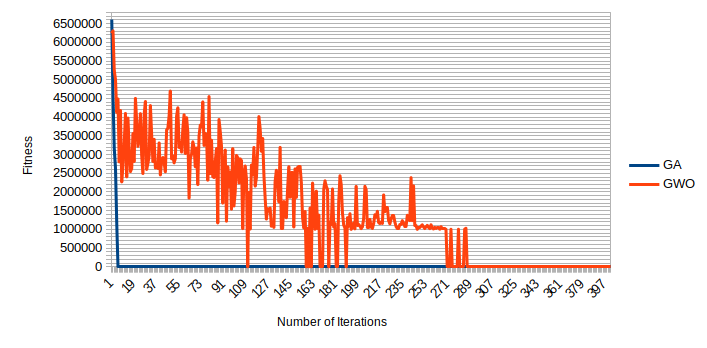
\includegraphics[scale=0.75]{./images/chap07-rd/gwo-sflp2-graph.png}
%\end{adjustwidth}
%\caption{Fitness graph of the best solutions of the competing GA approach, and our GWO approach using the SFLP-II data set.}
%\label{graph-ga-vs-gwo-sflp2}
%\end{figure}
%
%\begin{figure}[h!]
%\centering
%\begin{adjustwidth}{-0.1in}{}
%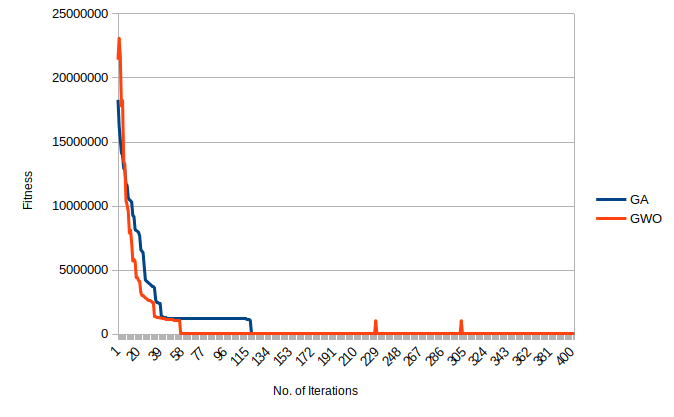
\includegraphics[scale=0.65]{./images/chap07-rd/gwo-msflp3-graph.png}
%\end{adjustwidth}
%\caption{Fitness graph of the best solutions of the competing GA approach, and our GWO approach using the mSFLP-III data set.}
%\label{graph-ga-vs-gwo-msflp3}
%\end{figure}

% TODO: Add figure of best generated solutions.\\

The performance of the GA approach in this study is definitely noteworthy. It produces the best solutions on average among the three approaches. However, based on the results, the GA approach does not scale well as the number of buildings increase, compared to our approach and the PSO approach. PSO definitely shows the best average runtimes. However, it produces the worst average fitness. For faster speed, we traded performance. This is where our approach shines. Our approach is the second best when it comes to solution quality as the problem scales higher. It is also the second best in terms of speed. This shows to us that our GWO approach provides a balance between speed and performance. Our approach also requires only a few parameters. We argue that this will simplify and speed up experimental setups and configuration in later studies and applications. Importantly, the results also indicate that there is promise in further exploring the applicability of the grey wolf optimization algorithm in solving the facility layout problem.

